\documentclass[12pt,oneside,a4paper,english]{article}
\usepackage[T1]{fontenc}
\usepackage[latin2]{inputenc}
\usepackage[margin=2.25cm,headheight=26pt,includeheadfoot]{geometry}
\usepackage[english]{babel}
\usepackage{listings}
\usepackage{color}
\usepackage{titlesec}
\usepackage{titling}
\usepackage[framed, numbered]{matlab-prettifier}
\usepackage{changepage}
\usepackage{amsmath,amssymb}
\usepackage{hyperref}
\usepackage{enumitem}
\usepackage{graphicx}
\usepackage{fancyhdr}
\usepackage{lastpage}
\usepackage{caption}
\usepackage{tocloft}
\usepackage{setspace}
\usepackage{multirow}
\usepackage{titling}
\usepackage{float}
\usepackage{comment}
\usepackage{booktabs}
\usepackage{indentfirst}
\usepackage{lscape}
\usepackage{booktabs,caption}
\usepackage[flushleft]{threeparttable}
\usepackage[english,intoc]{nomencl}
\usepackage{xcolor}
\usepackage{lipsum}
\usepackage{tabularx}

% --- handy macros for this assignment ---
\newcommand{\T}{\mathcal{T}}
\newcommand{\qimp}[1][t]{q^{\mathrm{imp}}_{#1}}
\newcommand{\qexp}[1][t]{q^{\mathrm{exp}}_{#1}}
\newcommand{\pimp}[1][t]{p^{\mathrm{imp}}_{#1}}        % effective import price
\newcommand{\pexp}[1][t]{p^{\mathrm{exp}}_{#1}}        % effective export price
\newcommand{\cpv}{c^{\mathrm{PV}}}
\newcommand{\Emin}{E^{\min}}
\newcommand{\lref}[1][t]{\hat{\ell}_{#1}}
\newcommand{\uL}{u^{L}}
\newcommand{\load}[1][t]{\ell_{#1}}
\newcommand{\pvprod}[1][t]{q^{\mathrm{PV}}_{#1}}
\newcommand{\Lmin}{L^{\min}}
\newcommand{\Lmax}{L^{\max}}
\newcommand{\PVmax}[1][t]{PV_{#1}^{\max}}
\newcommand{\tauexp}{\tau^{\mathrm{exp}}}
\newcommand{\tauimp}{\tau^{\mathrm{imp}}}
% dual variables of the hourly problem (Question 1.(b))
\newcommand{\lbal}[1][t]{\lambda_{#1}}
\newcommand{\muLlo}[1][t]{\underline{\mu}^{L}_{#1}}
\newcommand{\muLup}[1][t]{\overline{\mu}^{L}_{#1}}
\newcommand{\muPVlo}[1][t]{\underline{\mu}^{\mathrm{PV}}_{#1}}
\newcommand{\muPVup}[1][t]{\overline{\mu}^{\mathrm{PV}}_{#1}}
\newcommand{\muimp}[1][t]{\mu^{\mathrm{imp}}_{#1}}
\newcommand{\muexp}[1][t]{\mu^{\mathrm{exp}}_{#1}}
% multiplier of the minimum daily energy constraint (Question 3.(b)); one for the whole day
\newcommand{\muE}{\mu^{E}}
% battery of Question 3.(g)
\newcommand{\Ebat}{E^{\mathrm{bat}}}
\newcommand{\Pch}{P^{\mathrm{ch}}}
\newcommand{\Pdis}{P^{\mathrm{dis}}}
\newcommand{\etach}{\eta^{\mathrm{ch}}}
\newcommand{\etadis}{\eta^{\mathrm{dis}}}
\newcommand{\einit}{e^{\mathrm{init}}}
\newcommand{\pch}[1][t]{p^{\mathrm{ch}}_{#1}}
\newcommand{\pdis}[1][t]{p^{\mathrm{dis}}_{#1}}
\newcommand{\soc}[1][t]{e_{#1}}
\newcommand{\piend}{\pi^{\mathrm{end}}}

% --- nomenclature: all symbols are declared in sources/9_nomenclat.tex, with their units
\makenomenclature


% --- set footer and header ---
\pagestyle{fancy}
\fancyhf{}

% no first-line indent; paragraphs are separated by a small vertical gap instead
\setlength{\parindent}{0pt}
\setlength{\parskip}{0.6em plus 0.1em}
\title{46750 - Optimization in Modern Power Systems - Assignment 2} % to reference as \title, dont use \maketitle
\makeatletter\let\Title\@title\makeatother

% Code listings: Python (the recommended starter code is Python)
\lstset{language=Python,
basicstyle=\small\ttfamily,
keywordstyle=\color{blue},
commentstyle=\color{gray},
numbers=left,
numberstyle={\scriptsize\color{black}},
numbersep=0.5cm,
frame=single,
breaklines=true,
showstringspaces=false
}

\newlist{steps}{enumerate}{1}
\setlist[steps, 1]{leftmargin=1.5cm,label = Step \arabic*:}
\renewcommand{\headrulewidth}{1pt}
\renewcommand{\footrulewidth}{1pt}
\usepackage{xltabular}

\newcommand{\todo}[1]{{\color{red}\bfseries [TODO: #1]}}
% --- End of page settings ---


%\lhead{\Title}
\rhead{\nouppercase{\leftmark}} % \leftmark = current \section ("Question 1"); \rightmark = current \subsection
\lhead{\Title}
\rfoot{
\includegraphics[height=1.25cm]{root/logo.pdf}} % right header logo
\setlength\headheight{16pt}
\setlength{\footskip}{50pt}
\lhead{\Title} %rightH title
\cfoot{\thepage}

% --- End of page settings ---



\begin{document}
\pagenumbering{roman} 

\begin{titlepage}
\begin{center}
\vspace{2cm}
%\textsc{ Danmarks Tekniske Universitet}\\[1.5cm]

\includegraphics[width=0.4\textwidth]{root/dtu.png}~\\[1cm]
\vspace{2cm}

\vspace{2cm}

% Title
\hrule
\vspace{.5cm}
{ \LARGE \bfseries 46750 - Optimization in Modern Power Systems \\} % title of the report
\vspace{.25cm}
{\LARGE \textbf{Assignment 2}}
\vspace{.5cm}

\hrule
\vspace{1.5cm}

{\textsc{\textbf{Group    14}}}\\
\vspace{.5cm}
\centering

% add your name here
Alejandro Lopez Bermejo - s253272\\
Ignacio Marti Plaza - s253188\\
Erik Olsson - s262077\\
\vspace{1cm}

% TODO: repository link if you submit your code via GitHub (otherwise delete)
\textbf{Code repository:
\url{https://github.com/eriols0823/Optimization_assignment_2}}\\

\vspace{4cm}

\centering \today % Dags dato
\end{center}
\end{titlepage}

\newpage 


\newpage
\doublespacing
%\addcontentsline{toc}{section}{Table of Contents}
\renewcommand{\baselinestretch}{1}\normalsize
\tableofcontents
\renewcommand{\baselinestretch}{1}\normalsize
%\singlespacing
\thispagestyle{fancy} % force page style

\newpage

\section*{Group participation table}
\addcontentsline{toc}{section}{Group participation table}
% Fill in the contribution of each student, in percent, to each grading criterion and to the
% assignment as a whole. Each of the four criterion columns sums to 100%. The "Overall" column
% reflects the share of the total time spent by each student and need NOT be a weighted average of
% the criterion columns, since the criteria differ in the time they require. The overall share is
% the one used for the individual grade adjustment (see the assignment text).
\begin{table}[H]
  \centering
  \small
  \begin{tabular}{l>{\centering\arraybackslash}p{2.7cm}>{\centering\arraybackslash}p{1.8cm}>{\centering\arraybackslash}p{1.8cm}>{\centering\arraybackslash}p{2.2cm}>{\centering\arraybackslash}p{1.8cm}}
    \toprule
    \textbf{Student} & \textbf{Mathematical models} & \textbf{Writing} & \textbf{Code} & \textbf{Numerical results} & \textbf{Overall} \\
    \midrule
    Alejandro & 34\,\% & 25\,\% & 43\,\% & 18\,\% & 29\,\% \\
    Erik Olsson & 23\,\% & 30\,\% & 14\,\% & 37\,\% & 28\,\% \\
    Ignacio & 31\,\% & 28\,\% & 33\,\% & 43\,\% & 28\,\% \\
    \textbf{Sum} & 100\,\% & 100\,\% & 100\,\% & 100\,\% & 100\,\% \\
    \bottomrule
  \end{tabular}
  \caption{The percentages are based from all the questions, including the bonus question. Contribution of each group member to each grading criterion and to the assignment overall (in \% of the group total). The overall column reflects the time spent and is not a weighted average of the criterion columns.}
  \label{tab:participation}
\end{table}

% ------------------------------------------------------------ AI use disclosure
\section*{AI use disclosure}
\addcontentsline{toc}{section}{AI use disclosure}
% State which AI tools were used (e.g. ChatGPT, Claude, GitHub Copilot), for which tasks
% (e.g. debugging, code documentation, proofreading, brainstorming, plotting), and how the group
% checked the output (e.g. re-derived by hand, tested against a closed-form solution).
% Write "No AI tool was used." if that is the case. Using AI tools is allowed; not disclosing it is not.
\begin{table}[H]
  \centering
  \begin{tabularx}{\textwidth}{lXX}
    \toprule
    \textbf{Tool} & \textbf{Used for} & \textbf{How the output was verified} \\
    \midrule
        Claude (Claude Code and web)
    &
    Repository set-up; assistance writing and debugging the code; LaTeX typesetting, wording of
    the group's text and merging of drafts; explaining the brief and course concepts,
    discussing modeling choices and derivations.
    &
    Modelling choices were made by the group; derivations were checked by hand; LaTeX and code
    were compiled, run and checked by the group against the formulation.
    \\
    \midrule
    Gemini (Google)
    &
    Transcription of handwritten notes into typed text.
    &
    Checked against the handwritten originals and the lecture notes.
    \\
    \bottomrule
  \end{tabularx}
  \caption{AI tools used in this assignment.}
  \label{tab:ai}
\end{table}

\newpage 
\pagenumbering{arabic} 
\fancyfoot[C]{Page \thepage\ of \pageref{EndOfText}}



\newpage
% \printnomenclature (inside 9_nomenclat) prints its own "Nomenclature" heading, and the
% `intoc` option of the package adds it to the table of contents.
% Nomenclature of Assignment 2 (all questions). A static table (no makeindex needed), grouped by role.
% Add new symbols in the right block when a question introduces them; keep one row per symbol.
\section*{Nomenclature}
\addcontentsline{toc}{section}{Nomenclature}
\markboth{Nomenclature}{Nomenclature}
The notation of Assignment~1 is kept; the member index $i$ is added to every member quantity.
Energies are hourly, so kW and kWh/h are numerically interchangeable.

{\small
\begin{xltabular}{\textwidth}{@{}l X l@{}}
\toprule
\textbf{Symbol} & \textbf{Meaning} & \textbf{Unit} \\
\midrule
\endfirsthead
\toprule
\textbf{Symbol} & \textbf{Meaning} & \textbf{Unit} \\
\midrule
\endhead
\bottomrule
\endfoot
\multicolumn{3}{@{}l}{\textit{Sets and indices}} \\
$i\in\mathcal{M}$ & Members of the community (16 in the base case) & -- \\
$t\in\mathcal{T}$ & Hours of the day, $\{0,\dots,23\}$ & -- \\
$\mathcal{T}^{\mathcal{R}}$ & Hours in which the import of $\mathcal{R}$ exceeds the cap & -- \\
$\mathcal{X}_i$ & Feasible set of member $i$, constraints~\eqref{eq:member} & -- \\
\midrule
\multicolumn{3}{@{}l}{\textit{Market, grid and contract}} \\
$p_t$ & Day-ahead energy price & DKK/kWh \\
$\tau^{\mathrm{imp}}$, $\tau^{\mathrm{exp}}$ & Full grid tariffs on import and export & DKK/kWh \\
$p^{\mathrm{imp}}_t$, $p^{\mathrm{exp}}_t$ & Effective prices without contract, $p_t\pm\tau^{\mathrm{imp}/\mathrm{exp}}$ & DKK/kWh \\
$\tilde{p}^{\mathrm{imp}}_t$, $\tilde{p}^{\mathrm{exp}}_t$ & Discounted prices under a contract, \eqref{eq:ptilde} & DKK/kWh \\
$\beta^{\mathrm{DSO}}$ & Tariff discount of the contract, in $[0,1]$ & -- \\
$\alpha^{\mathrm{DSO}}$ & Penalty per kWh imported above the cap & DKK/kWh \\
$\overline{P}^{\mathrm{DSO}}_t$ & Hourly cap on the import at the connection point & kW \\
$f$ & Cap factor: $\overline{P}^{\mathrm{DSO}}_t=f\,E^{\mathcal{R}}/24$ (base 1.3) & -- \\
$E^{\mathcal{R}}$ & Daily import of the community without contract ($\mathcal{R}$) & kWh \\
$\kappa_i$ & Share of the cap of member $i$ in $\mathcal{I}$, $\sum_i\kappa_i=1$ & -- \\
\midrule
\multicolumn{3}{@{}l}{\textit{Member parameters}} \\
$\hat{\ell}_{i,t}$ & Reference (preferred) load & kWh/h \\
$\overline{\Delta}$ & Maximum hourly deviation from the reference load & kWh \\
$L^{\min}$, $L^{\max}$ & Minimum and maximum hourly load & kWh/h \\
$E^{\min}_i$ & Minimum daily energy (= daily reference energy) & kWh \\
$c^{L}_i$ & Slope of the linear disutility & DKK/kWh \\
$c^{\mathrm{PV}}$ & Marginal cost of PV production & DKK/kWh \\
$PV^{\max}_{i,t}$ & Available PV production & kWh/h \\
$E^{\mathrm{bat}}_i$ & Battery energy capacity & kWh \\
$P^{\mathrm{ch}}_i$, $P^{\mathrm{dis}}_i$ & Maximum charging and discharging power & kW \\
$\eta^{\mathrm{ch}}$, $\eta^{\mathrm{dis}}$ & Charging and discharging efficiencies & -- \\
$e^{\mathrm{init}}_i$ & State of charge at the start of the day & kWh \\
\midrule
\multicolumn{3}{@{}l}{\textit{Decision variables}} \\
$y_i$ & All decisions of member $i$ (load, deviations, PV, battery), $y_i\in\mathcal{X}_i$ & -- \\
$\ell_{i,t}$ & Load & kWh/h \\
$d^{+}_{i,t}$, $d^{-}_{i,t}$ & Deviation of the load above and below its reference, $\geq0$ & kWh/h \\
$q^{\mathrm{PV}}_{i,t}$ & PV production & kWh/h \\
$p^{\mathrm{ch}}_{i,t}$, $p^{\mathrm{dis}}_{i,t}$ & Battery charging and discharging power, $\geq0$ & kWh/h \\
$e_{i,t}$ & State of charge at the end of hour $t$ & kWh \\
$q_{i,t}$ & Net consumption, \eqref{eq:net} (free in sign) & kWh/h \\
$q^{\mathrm{imp}}_{i,t}$, $q^{\mathrm{exp}}_{i,t}$ & Import and export on the member's own meter ($\mathcal{R}$, $\mathcal{I}$) & kWh/h \\
$q^{\mathrm{exc}}_{i,t}$ & Import of member $i$ above its own cap ($\mathcal{I}$) & kWh/h \\
$P^{\mathrm{imp}}_t$, $P^{\mathrm{exp}}_t$ & Import and export of the community at the connection point & kWh/h \\
$P^{\mathrm{exc}}_t$ & Import of the community above the cap & kWh/h \\
$x_t$ & Internal price posted by the manager ($\mathcal{DP}$) & DKK/kWh \\
$\underline{x}_t$, $\overline{x}_t$ & Bounds of the posted price & DKK/kWh \\
$s_i$ & Violation of the individual rationality of member $i$ (soft variant) & DKK \\
$u_t$, $z_t$ & Binaries excluding simultaneous import/export and a penalty below the cap & -- \\
$M^{\mathrm{P}}$, $M^{\mathrm{D}}$ & Big-M constants of the primal and dual side of a complementarity pair (Appendix~A) & kWh, DKK/kWh \\
\midrule
\multicolumn{3}{@{}l}{\textit{Dual variables}} \\
$\lambda_t$ & Internal price of $\mathcal{C}$: dual of the internal balance~\eqref{eq:C_bal} & DKK/kWh \\
$\gamma_t$ & Cap price of $\mathcal{C}$: dual of~\eqref{eq:C_cap}, in $[0,\alpha^{\mathrm{DSO}}]$ & DKK/kWh \\
$\lambda^{\mathcal{R}}_{i,t}$, $\lambda^{\mathcal{I}}_{i,t}$ & Duals of the member's own balance in $\mathcal{R}$ and $\mathcal{I}$ & DKK/kWh \\
$\gamma_{i,t}$ & Dual of the individual cap in $\mathcal{I}$ & DKK/kWh \\
$\mu^{E}_i$ & Dual of the daily minimum: internal value of a kWh of daily need & DKK/kWh \\
$\nu_{i,t}$ & Dual of the deviation definition~\eqref{eq:dev}, $|\nu_{i,t}|\leq c^L_i$ ($\mathcal{DP}$) & DKK/kWh \\
$\underline{\mu}^{L}_{i,t}$, $\overline{\mu}^{L}_{i,t}$ & Duals of the hourly load bounds & DKK/kWh \\
$\underline{\mu}^{\mathrm{PV}}_{i,t}$, $\overline{\mu}^{\mathrm{PV}}_{i,t}$ & Duals of the PV bounds & DKK/kWh \\
$\psi_{i,t}$ & Dual of the state-of-charge balance ($-\psi_{i,t}$: value of stored energy) & DKK/kWh \\
$\underline{\mu}^{\mathrm{ch}},\overline{\mu}^{\mathrm{ch}},\underline{\mu}^{\mathrm{dis}},\overline{\mu}^{\mathrm{dis}},\underline{\mu}^{e},\overline{\mu}^{e}$ & Duals of the battery bounds (index $i,t$) & DKK/kWh \\
$\mu^{\mathrm{end}}_i$ & Dual of the end-of-day state of charge & DKK/kWh \\
$\xi_i$ & All dual variables of member $i$'s problem~\eqref{eq:DP_member} & -- \\
\midrule
\multicolumn{3}{@{}l}{\textit{Costs, payments and metrics}} \\
$K_i$ & Own cost of member $i$: disutility plus PV production cost, \eqref{eq:owncost} & DKK \\
$J^m_i$, $J^m$ & Cost of member $i$ and of the community in model $m$ & DKK \\
$W^{\mathcal{C}}$ & Welfare of the community, $-J^{\mathcal{C}}$ & DKK \\
$\Pi_i$ & Payment of member $i$ to the manager ($\sum_t\lambda_tq_{i,t}$ in $\mathcal{C}$, $\sum_tx_tq_{i,t}$ in $\mathcal{DP}$) & DKK \\
$\Phi_i$ & Dual objective of member $i$'s problem, $=\Pi_i+K_i$ by strong duality & DKK \\
$D$ & Bill of the DSO to the manager, \eqref{eq:bill} & DKK \\
$B$ & Manager's budget, $\sum_i\Pi_i-D$ & DKK \\
$J^{\mathrm{bench}}_i$ & Benchmark cost of member $i$ for individual rationality ($J^{\mathcal{R}}_i$ by default) & DKK \\
$\rho$ & Weight of the IR violation in the soft variant & DKK/DKK \\
$V^m$, $V^m_i$ & Gain of the community and of member $i$ against $\mathcal{R}$ & DKK \\
$X^m$ & Energy imported above the cap in model $m$ & kWh \\
$F^m$, $F^m_i$ & Flexibility: energy above the cap removed against $\mathcal{R}$ & kWh \\
$G^m$, $c^m$ & Tariff and penalty income of the DSO; its cost per kWh removed & DKK, DKK/kWh \\
\midrule
\multicolumn{3}{@{}l}{\textit{Models (variants named by superscripts)}} \\
$\mathcal{R}$, $\mathcal{I}$, $\mathcal{C}$ & No contract; individual contracts; community contract with central dispatch & -- \\
$\mathcal{F}_i(x)$ & Problem of member $i$ at posted prices $x$, \eqref{eq:DP_member} & -- \\
$\mathcal{DP}^{\mathrm{cap}}$, $\mathcal{DP}^{\mathrm{BB}}$, $\mathcal{DP}^{\mathrm{BB,IR}}$ & Pricing problem with the contract only; with budget balance; with individual rationality (Table~\ref{tab:DP_variants}) & -- \\
\end{xltabular}}


\newpage
\section{Question 1}
The question explores whether the members should sign a capacity limitation contract with the DSO. To answer this, three different optimization models based on different contracts will be explored. In model $\mathcal{R}$, no contract is signed and each member schedules independently at the full tariffs. In model $\mathcal{I}$, each member signs its own contract with a share of the capacity limit. The trade-off is that members get lower tariffs for import and export but have to pay a penalty if they exceed the limit. In this model, each member still acts independently. The last model $\mathcal{C}$ is similar to model $\mathcal{I}$, but instead a community manager coordinates the schedules of all members. A sensitivity analysis will also be made to better understand how different contract parameters affect the results.

First, a basic member model is introduced that is shared by all three models $\mathcal{R}$, $\mathcal{I}$ and $\mathcal{C}$. Each model is then presented mathematically. For $\mathcal{C}$ the settlement logic is also explained. After describing the problem class and defining the relevant metrics, the models are solved for the base case. The base case results are briefly analyzed before the sensitivity analysis is conducted. At last recommendations for the respective parties will be given.


\subsection{Models}
\subsubsection{Member model}
A big portion of the objective value as well as the constraints are shared in all models($\mathcal{R}$, $\mathcal{I}$ and $\mathcal{C}$). To not have to repeat them each time we will state them once here. 

Each member $i\in\mathcal{M}$ is an Assignment~1 consumer with a flexible load and potentially a PV system and battery.
The notations of Assignment~1 are kept in large, and the member index $i$ is added.
The decisions of member $i$ lie in the feasible set $\mathcal{X}_i$ defined by
\begin{subequations}\label{eq:member}
\begin{align}
& q_{i,t}=\ell_{i,t}+p^{\mathrm{ch}}_{i,t}-p^{\mathrm{dis}}_{i,t}-q^{\mathrm{PV}}_{i,t}, && \forall t\in\mathcal{T}, \label{eq:net}\\
& 0\le q^{\mathrm{PV}}_{i,t}\le PV^{\max}_{i,t}, && \forall t\in\mathcal{T}, \label{eq:pv}\\
& \ell_{i,t}-\hat{\ell}_{i,t}=d^{+}_{i,t}-d^{-}_{i,t},\qquad d^{+}_{i,t},\ d^{-}_{i,t}\ge 0, && \forall t\in\mathcal{T}, \label{eq:dev}\\
& \textstyle\sum_{t\in\mathcal{T}}\ell_{i,t}\ge E^{\min}_i && :\ \mu^{E}_i, \label{eq:emin}\\
& e_{i,t}=e_{i,t-1}+\eta^{\mathrm{ch}}p^{\mathrm{ch}}_{i,t}-p^{\mathrm{dis}}_{i,t}/\eta^{\mathrm{dis}},\qquad e_{i,-1}=e^{\mathrm{init}}_i, && \forall t\in\mathcal{T}, \label{eq:soc}\\
& 0\le e_{i,t}\le E^{\mathrm{bat}}_i,\qquad 0\le p^{\mathrm{ch}}_{i,t}\le P^{\mathrm{ch}}_i,\qquad 0\le p^{\mathrm{dis}}_{i,t}\le P^{\mathrm{dis}}_i, && \forall t\in\mathcal{T}, \label{eq:batbounds}\\
& \max\big(L^{\min},\hat{\ell}_{i,t}-\overline{\Delta}\big)\le \ell_{i,t}\le \min\big(L^{\max},\hat{\ell}_{i,t}+\overline{\Delta}\big), && \forall t\in\mathcal{T}, \label{eq:lbounds}\\
& e_{i,23}\ge e^{\mathrm{init}}_i. && \label{eq:eod}
\end{align}
\end{subequations}
Constraints~\eqref{eq:net}--\eqref{eq:batbounds} are the constraints of Assignment~1 with the member index $i$.
Two constraints are new.

Constraint~\eqref{eq:lbounds} replaces the load bounds of Assignment~1 and limits the deviation from the reference to $\overline{\Delta}$ in every hour.

Unlike Assignment~1 we do not value the stored energy at a price $\pi^{\mathrm{end}}$, instead with constraint~\eqref{eq:eod} we force it to be at a certain level at the end of the day.
%Such a price would differ between the models because their tariffs and internal prices differ.
%A cyclic state of charge keeps the models comparable.
The member's own cost is the disutility plus the PV production cost is given by:
\begin{equation}\label{eq:owncost}
K_i=\sum_{t\in\mathcal{T}}\Big[c^{L}_i\big(d^{+}_{i,t}+d^{-}_{i,t}\big)+c^{\mathrm{PV}}q^{\mathrm{PV}}_{i,t}\Big].
\end{equation}
The payments for grid energy are not part of $K_i$.
They differ between the models and are added in the following subsections.

\subsubsection{Model $\mathcal{R}$: no contract}

This is the scenario when there is no contract at all. Here each member schedules alone against the effective prices of Assignment~1:
\begin{subequations}\label{eq:R}
\begin{align}
\min_{x_i\in\mathcal{X}_i,\ q^{\mathrm{imp}}_{i},\ q^{\mathrm{exp}}_{i}\ge 0}\quad & J^{\mathcal{R}}_i=\sum_{t\in\mathcal{T}}\Big(p^{\mathrm{imp}}_t q^{\mathrm{imp}}_{i,t}-p^{\mathrm{exp}}_t q^{\mathrm{exp}}_{i,t}\Big)+K_i \label{eq:R_obj}\\
\text{s.t.}\quad & q_{i,t}=q^{\mathrm{imp}}_{i,t}-q^{\mathrm{exp}}_{i,t}, \qquad \forall t\in\mathcal{T}\ :\ \lambda^{\mathcal{R}}_{i,t}. \label{eq:R_bal}
\end{align}
\end{subequations}
Model $\mathcal{R}$ consists of one separate LP per member since no constraint links the members.
Its community cost is the sum of the members' costs $J^{\mathcal{R}}=\sum_i J^{\mathcal{R}}_i$.


\subsubsection{Model $\mathcal{I}$: individual contracts}

In model $\mathcal{I}$ each member signs the contract on its own meter.
The contract changes three things compared with $\mathcal{R}$.
First, the grid tariffs on all metered import and export are reduced by the discount $\beta^{\mathrm{DSO}}$:
\begin{equation}\label{eq:ptilde}
\tilde{p}^{\mathrm{imp}}_t=p_t+(1-\beta^{\mathrm{DSO}})\tau^{\mathrm{imp}},\qquad
\tilde{p}^{\mathrm{exp}}_t=p_t-(1-\beta^{\mathrm{DSO}})\tau^{\mathrm{exp}}.
\end{equation}
Second, member $i$ receives its own cap $\kappa_i\overline{P}^{\mathrm{DSO}}_t$.
The share $\kappa_i$ is proportional to the member's net import in $\mathcal{R}$ and $\sum_i\kappa_i=1$.
Third, every kWh imported above this cap costs the penalty $\alpha^{\mathrm{DSO}}$.
We call this energy the exceedance $q^{\mathrm{exc}}_{i,t}$.
Each member then solves
\begin{subequations}\label{eq:I}
\begin{align}
\min_{x_i\in\mathcal{X}_i,\ q^{\mathrm{imp}}_{i},\ q^{\mathrm{exp}}_{i},\ q^{\mathrm{exc}}_{i}\ge 0}\quad & J^{\mathcal{I}}_i=\sum_{t\in\mathcal{T}}\Big(\tilde{p}^{\mathrm{imp}}_t q^{\mathrm{imp}}_{i,t}-\tilde{p}^{\mathrm{exp}}_t q^{\mathrm{exp}}_{i,t}+\alpha^{\mathrm{DSO}}q^{\mathrm{exc}}_{i,t}\Big)+K_i \label{eq:I_obj}\\
\text{s.t.}\quad & q_{i,t}=q^{\mathrm{imp}}_{i,t}-q^{\mathrm{exp}}_{i,t}, \qquad \forall t\in\mathcal{T}\ :\ \lambda^{\mathcal{I}}_{i,t}, \label{eq:I_bal}\\
& q^{\mathrm{exc}}_{i,t}\ge q^{\mathrm{imp}}_{i,t}-\kappa_i\overline{P}^{\mathrm{DSO}}_t, \qquad \forall t\in\mathcal{T}\ :\ \gamma_{i,t}. \label{eq:I_cap}
\end{align}
\end{subequations}
Constraint~\eqref{eq:I_cap} makes $q^{\mathrm{exc}}_{i,t}$ at least the import above the cap.
The minimisation sets it exactly to this value since every kWh of exceedance is penalised.
The cap is therefore soft: a member may exceed it but pays $\alpha^{\mathrm{DSO}}$ for every extra kWh.
Its multiplier $\gamma_{i,t}$ is the value of one more kWh of cap and lies between $0$ and $\alpha^{\mathrm{DSO}}$.



\subsubsection{Model $\mathcal{C}$: community contract under central dispatch}
The community holds one contract at its single meter.
Only the import and export at the connection point pay the discounted prices. The capacity limit applies to the community as a whole, and energy exchanged between members behind the meter is free. The manager knows all members and dispatches them to minimise the community cost:

\begin{subequations}\label{eq:C}
\begin{align}
\min_{\substack{x_i\in\mathcal{X}_i\ \forall i\\ P^{\mathrm{imp}},\ P^{\mathrm{exp}},\ P^{\mathrm{exc}}\ge 0}}\quad & J^{\mathcal{C}}=\sum_{t\in\mathcal{T}}\Big(\tilde{p}^{\mathrm{imp}}_t P^{\mathrm{imp}}_t-\tilde{p}^{\mathrm{exp}}_t P^{\mathrm{exp}}_t+\alpha^{\mathrm{DSO}}P^{\mathrm{exc}}_t\Big)+\sum_{i\in\mathcal{M}}K_i \label{eq:C_obj}\\
\text{s.t.}\quad & \textstyle\sum_{i\in\mathcal{M}}q_{i,t}-\big(P^{\mathrm{imp}}_t-P^{\mathrm{exp}}_t\big)=0, \qquad \forall t\in\mathcal{T}\ :\ \lambda_t, \label{eq:C_bal}\\
& P^{\mathrm{exc}}_t\ge P^{\mathrm{imp}}_t-\overline{P}^{\mathrm{DSO}}_t, \qquad \forall t\in\mathcal{T}\ :\ \gamma_t. \label{eq:C_cap}
\end{align}
\end{subequations}
Constraint~\eqref{eq:C_bal} states that the members' net consumption equals the community's net import.
Its multiplier $\lambda_t$ is the internal price of energy.
It is the cost to the community of one more kWh consumed in hour $t$.
Constraint~\eqref{eq:C_cap} is the soft cap of $\mathcal{I}$ applied to the whole community.
Minimising $J^{\mathcal{C}}$ maximises the community welfare $W^{\mathcal{C}}=-J^{\mathcal{C}}$.
Since the manager has perfect information $\mathcal{C}$ is an upper bound on the value and flexibility the community can achieve.


%The KKT conditions at the connection point (Appendix~\ref{app:kkt}) give
%\begin{equation}\label{eq:lambda}
%\lambda_t=
%\begin{cases}
%\tilde{p}^{\mathrm{exp}}_t & \text{if } P^{\mathrm{exp}}_t>0,\\[2pt]
%\text{any value in } \big[\tilde{p}^{\mathrm{exp}}_t,\ \tilde{p}^{\mathrm{imp}}_t\big] & \text{if } P^{\mathrm{imp}}_t=P^{\mathrm{exp}}_t=0,\\[2pt]
%\tilde{p}^{\mathrm{imp}}_t & \text{if } %0<P^{\mathrm{imp}}_t<\overline{P}^{\mathrm{DSO}}_t,\\[2pt]
%\tilde{p}^{\mathrm{imp}}_t+\gamma_t \ \text{ with } \gamma_t\in[0,\alpha^{\mathrm{DSO}}] & \text{if } P^{\mathrm{imp}}_t=\overline{P}^{\mathrm{DSO}}_t,\\[2pt]
%\tilde{p}^{\mathrm{imp}}_t+\alpha^{\mathrm{DSO}} & \text{if } P^{\mathrm{imp}}_t>\overline{P}^{\mathrm{DSO}}_t.
%\end{cases}
%\end{equation}
%In hours where the cap binds the internal price exceeds $\tilde{p}^{\mathrm{imp}}_t$ by the congestion price $\gamma_t$.


Signing together never costs the community more than signing alone: $J^{\mathcal{C}}\le\sum_i J^{\mathcal{I}}_i$.
The manager could always copy the schedules of $\mathcal{I}$. In $\mathcal{C}$ these schedules cost no more. Imports and exports of different members cancel behind the meter. Unused cap of one member also covers the excess of another. The optimum of $\mathcal{C}$ is therefore at least as good as in $\mathcal{I}$.

\paragraph{Settlement.}
Each member pays the internal price $\lambda_t$ for its net consumption.
This payment replaces all grid charges the member would face alone:
\begin{equation}\label{eq:payment}
\Pi_i=\sum_{t\in\mathcal{T}}\lambda_t\,q_{i,t},\qquad J^{\mathcal{C}}_i=\Pi_i+K_i.
\end{equation}
A negative $\Pi_i$ is a payment to the member.
The manager pays the DSO bill $D$ and keeps the surplus $B$:
\begin{equation}\label{eq:bill}
D=\sum_{t\in\mathcal{T}}\Big(\tilde{p}^{\mathrm{imp}}_t P^{\mathrm{imp}}_t-\tilde{p}^{\mathrm{exp}}_t P^{\mathrm{exp}}_t+\alpha^{\mathrm{DSO}}P^{\mathrm{exc}}_t\Big),\qquad B=\sum_{i\in\mathcal{M}}\Pi_i-D.
\end{equation}
The budget is balanced if $B=0$. The settlement is reasonable for member $i$ if the member is not worse off than alone:
\begin{equation}\label{eq:ir}
J^{\mathcal{R}}_i-J^{\mathcal{C}}_i\ge 0 \qquad\text{and}\qquad J^{\mathcal{I}}_i-J^{\mathcal{C}}_i\ge 0 .
\end{equation}


\subsection{Problem class and duality }
Models $\mathcal{R}$, $\mathcal{I}$ and $\mathcal{C}$ are linear programs.
As in Assignment~1 strong duality holds and the KKT conditions are necessary and sufficient.
The multipliers are therefore exact marginal values.
This matters for the settlement because $\lambda_t$ is the cost to the community of one more kWh in hour $t$.
With linear costs $\lambda_t$ is not always unique.
This can happen when the community neither imports nor exports or when its import equals the cap.
\subsection{Metrics}

The metrics take three points of view: the community as a whole, the DSO and the members. Model $\mathcal{R}$ is the reference. Contracts $\mathcal{I}$ and $\mathcal{C}$ are compared through their values of the same metric.

\paragraph{Community.}
The community gain is the cost the community saves with contract $m \in \{\mathcal{I},\mathcal{C}\}$ compared with $\mathcal{R}$:
\begin{equation}
    V^m = J^{\mathcal{R}} - J^m
    \label{eq:gain}
\end{equation}
Here $J^m$ is the optimal objective value of model $m$ in DKK. It is the grid bill for energy, tariffs and penalties plus the own costs $K_i$ of all members. The difference $V^{\mathcal{C}} - V^{\mathcal{I}}$ is what signing together is worth compared with signing alone.

\paragraph{DSO.}
The DSO wants less import above its cap $\overline{P}_t^{\mathrm{DSO}}$. The energy imported above the cap in model $m$ is
\begin{equation}
    X^m = \sum_t \max\left(0,\, P_t^m - \overline{P}_t^{\mathrm{DSO}}\right)
    \label{eq:exceedance}
\end{equation}
where $P_t^m$ is the sum of the members' imports in $\mathcal{R}$ and $\mathcal{I}$ and the import at the connection point in $\mathcal{C}$. The flexibility in kWh is the energy above the cap that contract $m$ removes:
\begin{equation}
    F^m = X^{\mathcal{R}} - X^m
    \label{eq:flexibility}
\end{equation}
The DSO pays for this flexibility through lower grid charges. Its cost per kWh removed is
\begin{equation}
    c^m = \frac{G^{\mathcal{R}} - G^m}{F^m}
    \label{eq:dso_cost}
\end{equation}
where $G^m$ in DKK is the DSO's income from tariffs and penalties in model $m$.


\paragraph{Members.}
The gain of member $i$ is defined like the community gain, but now calculated for each member instead of as a sum:
\begin{equation}
    V_i^m = J_i^{\mathcal{R}} - J_i^m
    \label{eq:gain_member}
\end{equation}
In $\mathcal{R}$ and $\mathcal{I}$ the member cost $J_i^m$ is the member's own grid bill plus $K_i$. In $\mathcal{C}$ it is the payment $\Pi_i$ from the settlement plus $K_i$. The manager's budget $B$ is the payments collected minus the DSO bill. The member gains add up to $\sum_i V_i^{\mathcal{C}} = V^{\mathcal{C}} - B$ because the manager keeps $B$.

The flexibility of member $i$ is how much it reduces its net consumption in the hours $\mathcal{T}^{\mathcal{R}}$ where $\mathcal{R}$ exceeds the cap:
\begin{equation}
    F_i^{\mathcal{C}} = \sum_{t \in \mathcal{T}^{\mathcal{R}}} \left(q_{i,t}^{\mathcal{R}} - q_{i,t}^{\mathcal{C}}\right)
    \label{eq:flexibility_member}
\end{equation}
Comparing $V_i^{\mathcal{C}}$ with $F_i^{\mathcal{C}}$ shows whether the members who provide flexibility are paid for it.

The community and DSO metrics are used in the sensitivity analysis. The member metrics and $B$ are used in the settlement analysis.

\subsection{Base case}
\label{basecase}
The base case shows what each contract is worth to the community and the DSO under the terms of the assignment on day d1.
These are $\beta^{\mathrm{DSO}}=0.75$ and $\alpha^{\mathrm{DSO}}=10$~DKK/kWh and a cap of 9.39~kW in every hour. Model $\mathcal{R}$ reproduces the reference values given in the contract file.
Its cost is 398.24~DKK and its daily import is 173.4~kWh with a peak of 27.6~kW.
The limit case also holds: central dispatch without a contract gives the same result as $\mathcal{R}$. 
Table~\ref{tab:base} summarises the base case.

\begin{table}[htbp]
\centering
\caption{Base case on day d1 with $\mathcal{R}$ as reference.}
\label{tab:base}
\small
\begin{tabular}{@{}lrrr@{}}
\toprule
 & $\mathcal{R}$ & $\mathcal{I}$ & $\mathcal{C}$\\
\midrule
Community cost $J^{m}$ [DKK] & 398.2 & 480.7 & 372.2\\
Earnings $V^{m}$ [DKK] & -- & $-82.4$ & $\mathbf{26.1}$\\
\midrule
Tariffs [DKK] & 93.9 & 22.4 & 24.7\\
Penalty [DKK] & 0.0 & 42.9 & 0.0\\
Disutility [DKK] & 3.7 & 107.1 & 47.4\\
Disutility of the L4 members [DKK] & 0.0 & 56.6 & 0.8\\
\midrule
Energy above the cap $X^{m}$ [kWh] & 66.4 & 4.3 & $\mathbf{0.0}$\\
Hours above the cap & 9 & 11 & 0\\
Peak import [kW] & 27.6 & 11.1 & 9.4\\
DSO cost per kWh removed [DKK/kWh] & -- & 0.46 & 1.04\\
\bottomrule
\end{tabular}

\vspace{3pt}
{\footnotesize L4 denotes the four members with the stiffest load and a disutility slope of $c^{L}_i=2.0$~DKK/kWh.}
\end{table}


\paragraph{No contract.}
Without a contract the import exceeds the cap in 9 hours and mostly around the midday peak of the reference load.
Nobody pays for this congestion because $\mathcal{R}$ has no cap.
The members barely shift load as the low disutility of 3.7 DKK shows.

\paragraph{Individual contracts.}
Individual contracts cut the energy above the cap from 66.4 to 4.3~kWh but cost the community 82.4~DKK more than $\mathcal{R}$.
The tariff saving of 71.5~DKK cannot cover 42.9~DKK in penalties and 103.4~DKK of extra disutility. The four L4 members alone carry 56.6~DKK of this disutility.

\paragraph{Community contract.}
The community contract removes all energy above the cap and saves 26.1~DKK compared with $\mathcal{R}$.
The tariff saving of 69.2~DKK now outweighs the extra disutility of 43.7~DKK.
The L4 members carry only 0.8~DKK of it against 56.6~DKK in $\mathcal{I}$ as the more flexible members shift instead.


\paragraph{DSO perspective}
The DSO gives up 1.04~DKK of income per kWh removed in $\mathcal{C}$ but only 0.46~DKK in $\mathcal{I}$. It is cheaper in $\mathcal{I}$ because the members pay 42.9~DKK in penalties to the DSO. However, in the base case of $\mathcal{I}$ informed members would never sign it. Whether 1.04~DKK per kWh is cheap depends on the cost of reinforcing the feeder. Whether every member gains under $\mathcal{C}$ is analyzed in the settlement section.

\subsection{Sensitivity Analysis}\label{sec:sensitivity}
The base case covers only one set of contract terms.
This section shows under which discount and cap each contract pays off for the community and how much flexibility it gives the DSO.
The two terms are varied together because the discount the community needs depends on how tight the cap is.
The cap follows the rule of the assignment
\begin{equation}
    \overline{P}^{\mathrm{DSO}}_t = f\,\frac{E^{\mathcal{R}}}{24}
    \label{eq:cap}
\end{equation}
where $E^{\mathcal{R}}$ is the daily import of $\mathcal{R}$ and $f$ is the cap factor.
The cap is thus $f$ times the average hourly import without contract.
A smaller $f$ means a tighter cap.
The discount $\beta^{\mathrm{DSO}}$ is varied from 0 to 0.95 in steps of 0.05 and $f$ from 1.0 to 4.0 in steps of 0.1.
The range goes from a very tight cap to one above the peak import of $\mathcal{R}$.
This gives 620 combinations around the base case of $\beta^{\mathrm{DSO}}=0.75$ and $f=1.3$.
The penalty stays at $\alpha^{\mathrm{DSO}}=10$~DKK/kWh in all runs.



\subsubsection{Hypotheses}
A tighter cap forces more load shifting and should therefore need a larger discount before the community contract pays off.
The same should hold for individual contracts, which should need an even larger discount as no member can use the unused cap of others.
The flexibility of both contracts should depend on the cap alone because the penalty is much larger than any tariff saving.

\subsubsection{Results and Discussion}

Figure~\ref{fig:sweep_earnings} shows the community earnings over the discount and the cap.
The discount the community needs grows quickly as the cap tightens. At the base cap $f=1.3$ the community contract beats $\mathcal{R}$ from $\beta^{\mathrm{DSO}}=0.50$.
At $f=1.1$ it needs 0.85 and at $f=1.0$ no discount up to 0.95 is enough. For loose caps with $f\geq 3.4$ the contract pays off even without a discount because members trade behind the meter.

\begin{figure}[htbp]
\centering
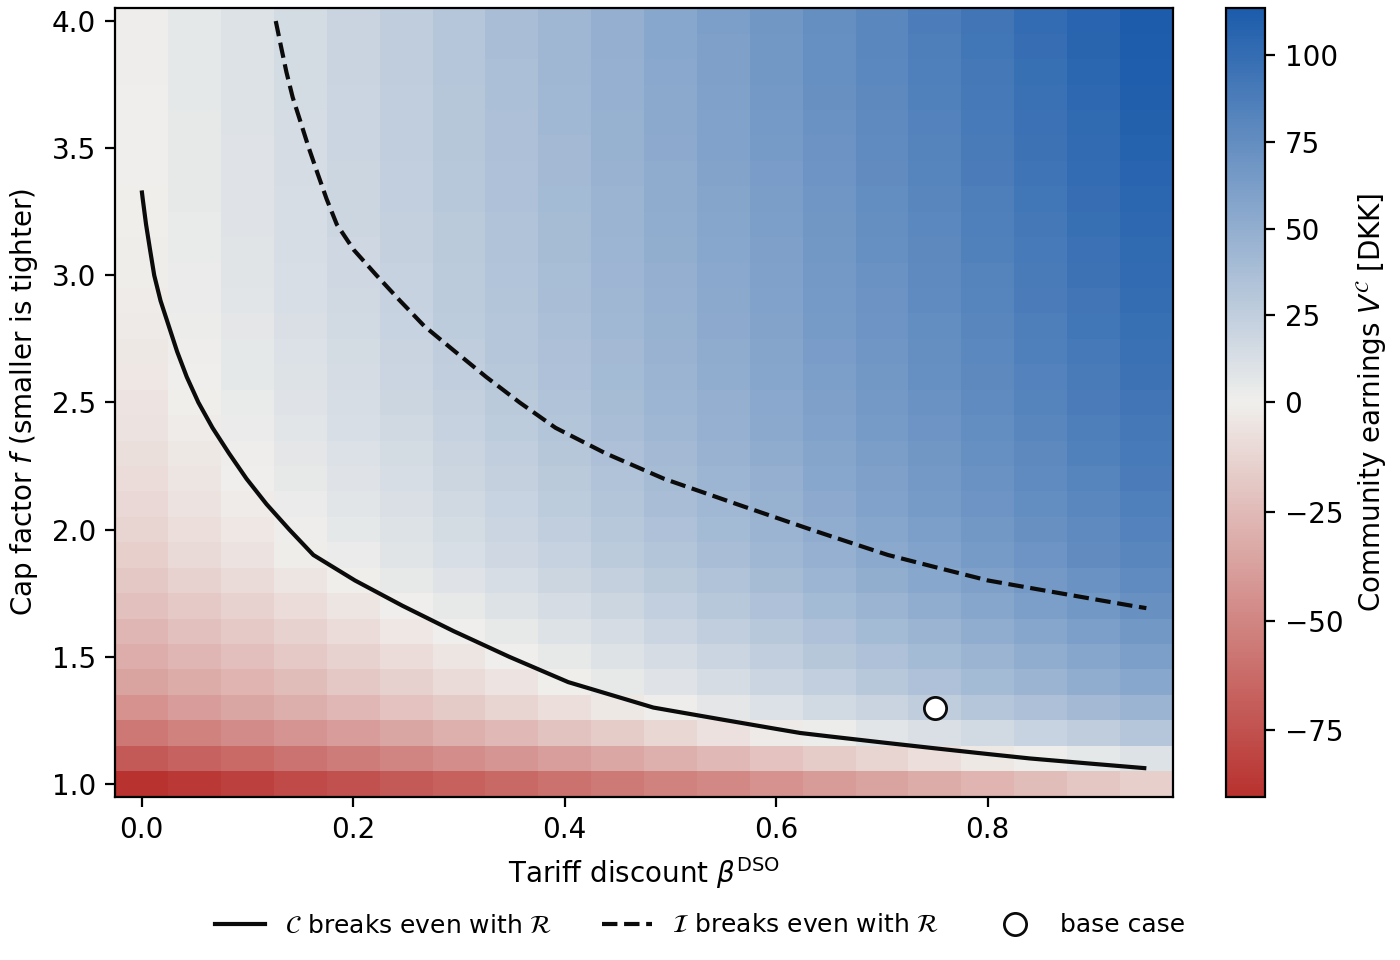
\includegraphics[width=0.8\linewidth]{figures/Q1/q1_sweep_earnings.png}
\caption{Community earnings $V^{\mathcal{C}}$ compared with $\mathcal{R}$. Blue means the community contract pays off}
\label{fig:sweep_earnings}
\end{figure}

Individual contracts only pay off above the dashed line in the dark blue region where the community contract already earns a lot.
They never pay off for $f\leq 1.6$ and still need a discount of 0.15 at $f=4.0$ where the cap no longer binds the community. Their slices thus keep binding some members.

Across all 620 combinations the flexibility of both contracts changes by less than 0.01~kWh with the discount. Figure~\ref{fig:sweep_flex} therefore shows flexibility against the cap factor alone. Due to the high penalty the community contract leaves less than 0.01~kWh above the cap in every combination. Its flexibility thus equals the congestion under $\mathcal{R}$. Individual contracts provide slightly less flexibility since each member is restricted separately rather than at the community level.
At the base cap they remove 62.1~kWh compared to 66.4~kWh for $\mathcal{C}$.
The two contracts provide equal flexibility for $f \geq 2.5$.
The DSO therefore gets nearly the same flexibility from both contracts.


\begin{figure}[htbp]
\centering
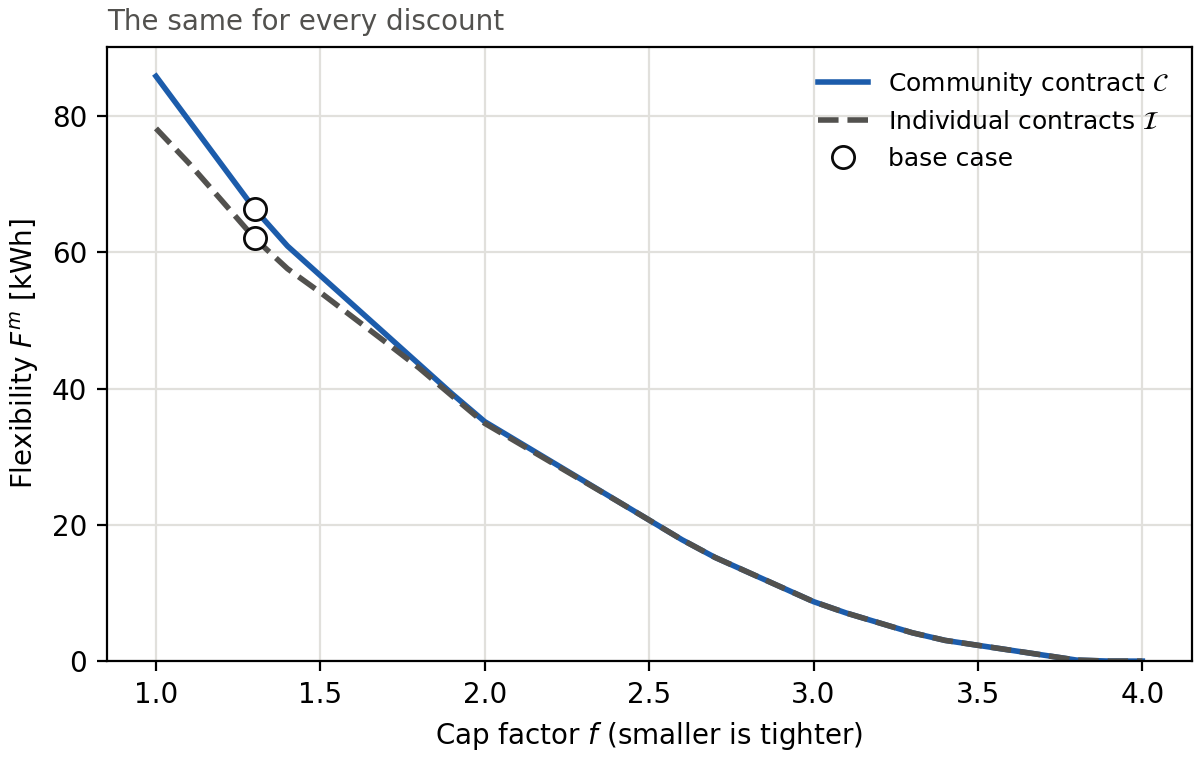
\includegraphics[width=0.7\linewidth]{figures/Q1/q1_sweep_flexibility.png}
\caption{Flexibility $F^m$ for the DSO. Both contracts give the same flexibility for every discount. Individual contracts remove slightly less when the cap is tight.}
\label{fig:sweep_flex}
\end{figure}

Together the two figures show the trade-off of the DSO.
The cap decides how much flexibility the DSO gets and the discount decides whether the community accepts.
From $f=2.0$ to $f=1.3$ the flexibility grows by 31.2~kWh for 0.35 more discount.
From $f=1.3$ to $f=1.1$ the same extra discount buys only 13.0~kWh.
Each extra kWh of flexibility thus becomes more expensive for the DSO as the cap tightens.

The figures thus confirm the hypotheses on the discount the community contract needs and on the flexibility.
The hypothesis on individual contracts holds only for the cap since a small discount is enough once the cap is loose.

\subsection{Settlement in $\mathcal{C}$}\label{sec:settlement}

The settlement is analysed on the base case of Section~\ref{basecase}, where the community contract $\mathcal{C}$ pays off for the community as a whole. This section shows whether every member also gains and whether the manager's budget is balanced. Under the settlement~\eqref{eq:payment}, all members pay the same internal price $\lambda_t$ in a given hour. This price is the dual of the balance~\eqref{eq:C_bal} and equals the cost to the community of one more kWh in hour $t$. It is unique in 23 of 24 hours. In the remaining hour no member consumes or produces energy, so its price affects no payment. Re-solving $\mathcal{C}$ with slightly more and slightly less consumption of each member gives the highest and lowest payment it could face. The two are equal for every member, so the results do not depend on which dual solution the solver returns.


In the hours where the cap binds and the community would like to import more, the internal price lies above the import price.
Since moving load to another hour is cheaper than the penalty, the community keeps its import at the cap.
One more kWh in such an hour therefore only fits if another member gives up its preferred schedule and moves one kWh out.
The internal price includes the discomfort of that member, making it the price at which the member is just willing to move.
In hour 11 even the stiff L4 loads must move, and the internal price reaches 5.41~DKK/kWh while the import itself costs only 1.225~DKK/kWh.

The manager collects 342.77~DKK at the internal prices but pays the DSO only 179.00~DKK at the discounted import price.
The difference of $B=163.77$~DKK stays with the manager, so the budget is not balanced.
Together the members thus lose 137.69~DKK, although the community as a whole gains 26.08~DKK.

\begin{figure}[H]
\centering
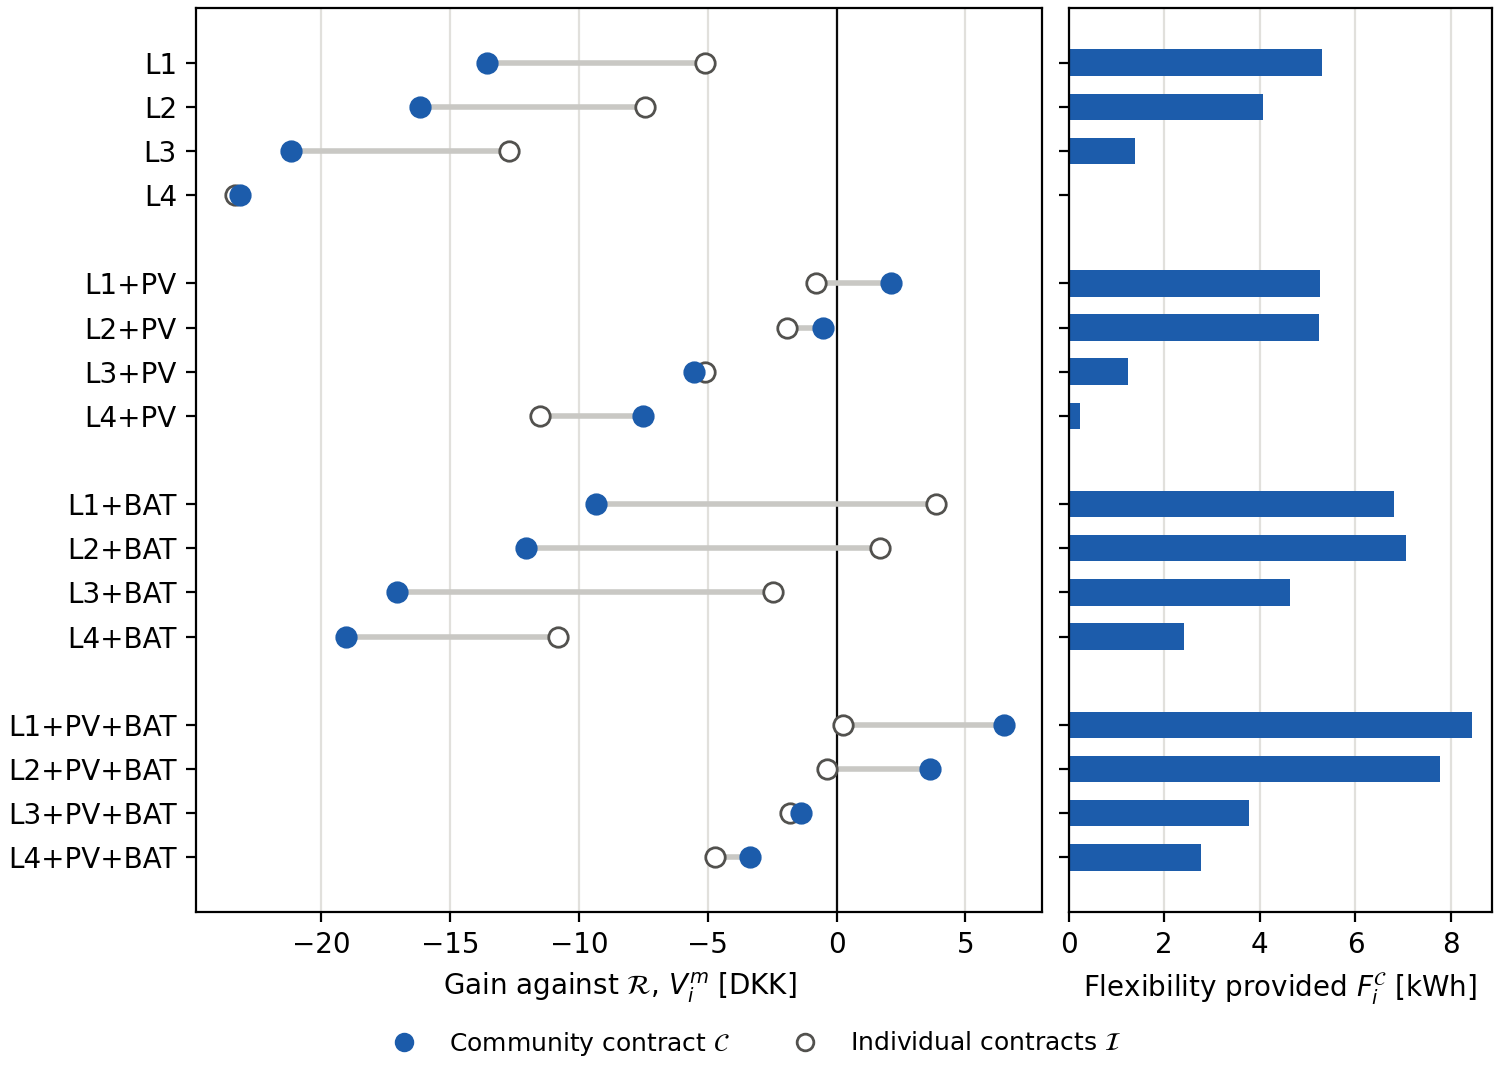
\includegraphics[width=0.85\linewidth]{figures/Q1/q1_settlement.png}
\caption{Gain of each member against $\mathcal{R}$ under the community contract (filled) and individual contracts (hollow), with the flexibility it provides in $\mathcal{C}$ (right).}
\label{fig:settlement}
\end{figure}

Figure~\ref{fig:settlement} shows the gain of every member compared with $\mathcal{R}$.
Only 3 of 16 members are not worse off than $\mathcal{R}$, and all of them own PV and have a flexible load(L1 or L2).
They sell PV energy to other members at the high internal price.
Members who cannot move their load still pay this price, as it is the same for everyone.
The stiff L4 member without assets therefore loses the most with 23.16~DKK.
Compared with $\mathcal{I}$, 8 of 16 members are not worse off under $\mathcal{C}$. All battery owners without PV would however prefer $\mathcal{I}$. These battery owners provide 5.23~kWh of flexibility on average but still lose 14.38~DKK. This is probably because the battery is worth less to its owner in $\mathcal{C}$. In $\mathcal{I}$ it saves the penalty on the owner's own small cap.
In $\mathcal{C}$ the cap is shared, so the battery competes with the flexibility of all other members and only earns the spread of the internal price.

PV owners without battery provide only 2.99~kWh and lose just 2.86~DKK.
Under the dual settlement, owning PV thus matters more than providing flexibility.

\subsection{Summary and Recommendations}
This section summarizes the main findings and gives recommendations to the members, manager and DSO.

Figure~\ref{fig:settlement} shows that an individual contract is the best option for only two members, the L1 and L2 members with only a battery. Since all members take the same decision, individual contracts are still not relevant as they cost the community 82.4~DKK and never pay off for $f\leq 1.6$ in Section~\ref{sec:sensitivity}. The community contract is the best option for three members, the L1 member with PV and the L1 and L2 members with PV and battery. It earns the community as a whole 26.08~DKK, but the other 13 members lose under it as the manager keeps a surplus of 163.77~DKK. A community contract therefore needs a joint decision that binds every member, since those who prefer $\mathcal{I}$ or $\mathcal{R}$ would otherwise refuse it. For 11 of 16 members $\mathcal{R}$ is the best option, so a majority vote would keep the members in $\mathcal{R}$ under the current settlement. The community contract would only become relevant if the manager paid the surplus back to the members in some fitting way. As the community gains as a whole, such a repayment could compensate every member who loses. 

The manager prefers the community contract, as it keeps the surplus of 163.77~DKK. Compensating the 13 members who lose would cost 149.92~DKK, so the manager would still keep 13.85~DKK in that case. Sharing part of the surplus can therefore suit both the manager and the members.

The goal of the DSO is to remove enough congestion at the lowest possible discount. Section~\ref{sec:sensitivity} shows that a tighter cap gives more flexibility but requires a larger discount, from 0.50 at $f=1.3$ to 0.85 at $f=1.1$. At $f=1.0$ no discount up to 0.95 is enough. The DSO should therefore choose the loosest cap that still relieves its feeder the desired amount, with a discount just large enough for the community to be formed. This only holds if the manager shares the surplus, as the members would otherwise not sign.
.





\newpage
\section{Question 2}
% =====================================================================================================
% Question 2 -- Can price signals achieve what the central dispatch does?                  (Alejandro)
% Code: src/pricing.py (model), src/q2.py (experiments). Every number below comes from one of
%   python main.py --q2 validate | steps | indifference | sensitivity
% =====================================================================================================
In Question~1 the manager could switch every appliance of the community on and off.
We now take this power away.
Once a day, after the day-ahead prices and the cap are known, the manager posts one internal price $x_t$ for every hour, the same for all members, and each member then schedules its own appliances against these prices, exactly as the consumer of Assignment~1 did.
The manager still pays the DSO for the exchange at the connection point and knows perfectly how every member responds.
We ask how much of the value and flexibility of $\mathcal{C}$ these prices can recover, whether the same prices can also balance the manager's budget and leave every member better off than alone, and what these two requirements cost the community.

\subsection{Models}

\subsubsection{Members: best response to posted prices}
Member $i$ keeps the feasible set $\mathcal{X}_i$ of~\eqref{eq:member} and the own cost $K_i$ of~\eqref{eq:owncost}.
Given the posted prices $x=(x_t)_{t\in\mathcal{T}}$, it chooses its decisions $y_i$ (load, deviations, PV and battery) by solving
\begin{equation}\label{eq:DP_member}
\mathcal{F}_i(x):\qquad \min_{y_i\in\mathcal{X}_i}\ J^{\mathcal{DP}}_i=\sum_{t\in\mathcal{T}}x_t\,q_{i,t}+K_i .
\end{equation}
Compared with $\mathcal{R}$, the member no longer has a meter of its own.
The import and export variables, the balance~\eqref{eq:R_bal}, the tariffs and the penalty all leave its problem, and the two prices $p^{\mathrm{imp}}_t>p^{\mathrm{exp}}_t$ become a single price $x_t$ on its net consumption.
Since the price only enters the objective, the manager changes what each member optimizes but never what it can do.

Buying and selling at the same price has three consequences.
A kWh of PV is worth $x_t$ whether it is used at home, sold to a neighbour or exported, so self-consumption earns no premium and the PV runs whenever $x_t\geq c^{\mathrm{PV}}$.
The battery only reacts to price differences and moves energy from hour $t$ to hour $s$ when $\eta^{\mathrm{ch}}\eta^{\mathrm{dis}}x_s>x_t$.
For the manager, the budget of hour $t$ becomes $(x_t-\tilde{p}^{\mathrm{imp}}_t)P^{\mathrm{imp}}_t-(x_t-\tilde{p}^{\mathrm{exp}}_t)P^{\mathrm{exp}}_t-\alpha^{\mathrm{DSO}}P^{\mathrm{exc}}_t$, so it collects a rent whenever the price of an importing hour exceeds the discounted import price.

Problem~\eqref{eq:DP_member} is a linear program, and its KKT conditions are listed in Appendix~A.
For the load they give the three regimes of Assignment~1.
With $\mu^E_i$ the multiplier of the daily minimum, the load stays at its reference while $|x_t-\mu^E_i|<c^L_i$ and moves to one of its bounds otherwise.
When $|x_t-\mu^E_i|=c^L_i$ the member is indifferent, and its best response is a set rather than a single schedule.

\subsubsection{Manager: welfare-maximizing prices}
The manager chooses the prices and the exchange at the connection point, anticipating how every member will respond:
\begin{subequations}\label{eq:DP}
\begin{align}
\min_{\substack{x,\ P^{\mathrm{imp}},P^{\mathrm{exp}},P^{\mathrm{exc}}\geq 0\\ (y_i)_{i\in\mathcal{M}}}}\quad & J^{\mathcal{DP}}=\sum_{t\in\mathcal{T}}\Big(\tilde{p}^{\mathrm{imp}}_tP^{\mathrm{imp}}_t-\tilde{p}^{\mathrm{exp}}_tP^{\mathrm{exp}}_t+\alpha^{\mathrm{DSO}}P^{\mathrm{exc}}_t\Big)+\sum_{i\in\mathcal{M}}K_i \label{eq:DP_obj}\\
\text{s.t.}\quad & \eqref{eq:C_bal},\ \eqref{eq:C_cap}, \qquad \underline{x}_t\leq x_t\leq\overline{x}_t \qquad \forall t\in\mathcal{T}, \label{eq:DP_upper}\\
& y_i\in\arg\min\ \mathcal{F}_i(x) \qquad \forall i\in\mathcal{M}. \label{eq:DP_lower}
\end{align}
\end{subequations}
The objective~\eqref{eq:DP_obj} is the welfare of $\mathcal{C}$.
The internal payments $\sum_tx_tq_{i,t}$ are transfers between the members and the manager, so they cancel out.
The manager therefore acts in the interest of the community but is indifferent to how the welfare is shared: the prices only matter through the dispatch they induce.
We bound the prices by $\underline{x}_t=0$, since a negative price would pay members to waste energy, and by $\overline{x}_t=\max_s\tilde{p}^{\mathrm{imp}}_s+\alpha^{\mathrm{DSO}}$, since no kWh can ever cost the community more.
Both bounds contain every value that $\lambda_t$ took in Question~1.

Two properties follow directly from this formulation.
First, $J^{\mathcal{DP}}\geq J^{\mathcal{C}}$, because~\eqref{eq:DP_lower} restricts the dispatch of $\mathcal{C}$ to the responses the members are willing to give.
Second, the dual prices $\lambda_t$ of~\eqref{eq:C_bal} attain $J^{\mathcal{C}}$.
The KKT conditions of $\mathcal{C}$ separate member by member when every member sees $\lambda_t$, so the dispatch of $\mathcal{C}$ is a best response of every member to these prices.
This is the competitive-equilibrium argument behind uniform marginal pricing in market clearing.
One uniform price per hour is therefore enough to reproduce $\mathcal{C}$.
That price is not unique, though, and nothing in~\eqref{eq:DP} protects the members.

\paragraph{Solution concept.}
Problem~\eqref{eq:DP} is a Stackelberg game in which the manager leads and the members follow.
When a member is indifferent, \eqref{eq:DP_lower} lets the manager pick the response it prefers among the member's optimal ones, which makes~\eqref{eq:DP} an optimistic bilevel problem.
We return to this assumption in Section~\ref{sec:q2_indifference}.

\subsubsection{Single-level reformulation}
Each $\mathcal{F}_i(x)$ is a linear program, so its KKT conditions describe its set of optimal responses exactly and can replace~\eqref{eq:DP_lower}.
The stationarity conditions are linear in the prices and the duals, because $x_t$ never multiplies a variable there.
What remains non-convex are the complementarity conditions $0\leq a\perp b\geq0$.
We write each of them with one binary $u$ as $a\leq M^{\mathrm{P}}u$ and $b\leq M^{\mathrm{D}}(1-u)$.
The constants $M^{\mathrm{P}}$ follow from the bounds of $\mathcal{X}_i$.
For the load and the PV, the constants $M^{\mathrm{D}}$ follow from the KKT conditions themselves, so they cut off no response (Appendix~A).
For the battery we use $M^{\mathrm{D}}=50$~DKK/kWh and check after every solve that no dual reaches it.
The objective~\eqref{eq:DP_obj} contains no product of a price and a quantity, so the variant with the contract only, $\mathcal{DP}^{\mathrm{cap}}$, needs no further step.
The requirements below do contain the payments $\Pi_i=\sum_tx_tq_{i,t}$, which are bilinear.
Strong duality of $\mathcal{F}_i(x)$ gives $\Pi_i+K_i=\Phi_i(\xi_i)$, the dual objective of member $i$ (Appendix~A).
$\Phi_i$ is linear in the duals $\xi_i$, because the prices only appear in the dual constraints.
The result is a mixed-integer linear program.

\subsubsection{Requirements and variants}
\paragraph{Budget balance.}
The manager is a non-profit entity, so the payments it collects must equal the DSO bill $D$ of~\eqref{eq:bill}:
\begin{equation}\label{eq:DP_BB}
\sum_{i\in\mathcal{M}}\big(\Phi_i(\xi_i)-K_i\big)=D .
\end{equation}
We use an equality rather than an inequality because~\eqref{eq:DP_obj} does not see the transfers: with an inequality, the surplus would be arbitrary among the optimal solutions.
The equality has a side effect, however.
The manager could balance its budget by wasting money at the meter, importing and exporting in the same hour or paying the penalty below the cap.
Two binaries per hour, $u_t$ and $z_t$, rule this out through $P^{\mathrm{imp}}_t\leq Mu_t$, $P^{\mathrm{exp}}_t\leq M(1-u_t)$, $P^{\mathrm{exc}}_t\leq Mz_t$ and $P^{\mathrm{exc}}_t\leq P^{\mathrm{imp}}_t-\overline{P}^{\mathrm{DSO}}_t+M(1-z_t)$.

\paragraph{Individual rationality.}
No member may end up worse off than in its benchmark:
\begin{equation}\label{eq:DP_IR}
\Phi_i(\xi_i)\leq J^{\mathrm{bench}}_i \qquad \forall i\in\mathcal{M}.
\end{equation}
Both sides contain the same components as~\eqref{eq:ir}: payments, disutility and PV production cost, with the same end-of-day state of charge.
Our benchmark is $\mathcal{R}$, because signing nothing is the one option every member always keeps.
A stricter variant, $\mathrm{IR}^{\mathcal{RI}}$, uses $\min(J^{\mathcal{R}}_i,J^{\mathcal{I}}_i)$ under the same contract terms.

\paragraph{Infeasibility.}
A single price per hour may not be able to satisfy both requirements, so we extend the same model in two ways.
In the soft variant $\mathcal{DP}^{\mathrm{BB,IR,soft}}$, each member's benchmark in~\eqref{eq:DP_IR} is relaxed by a slack $s_i\geq0$, and $\rho\sum_is_i$ with $\rho=10^3$ is added to~\eqref{eq:DP_obj}.
The members with $s_i>0$ are the ones blocking, and $\sum_is_i$ is what would have to be given up to satisfy them.
With price discrimination, $x_t$ is replaced by one price vector per asset class ($\mathcal{DP}^{\cdot,\mathrm{asset}}$, four vectors) or per member ($\mathcal{DP}^{\cdot,\mathrm{member}}$), which tells us how many price signals the requirements actually need.
Table~\ref{tab:DP_variants} summarizes the variants.

\begin{table}[htbp]
\centering
\caption{Variants of the pricing problem, all built as one parametrized model (\texttt{src/pricing.py}).}
\label{tab:DP_variants}
\small
\begin{tabular}{@{}lll@{}}
\toprule
Variant & Constraints added to \eqref{eq:DP} & Prices\\
\midrule
$\mathcal{DP}^{\mathrm{cap}}$ & -- & one per hour\\
$\mathcal{DP}^{\mathrm{BB}}$ & \eqref{eq:DP_BB} and the binaries $u_t,z_t$ & one per hour\\
$\mathcal{DP}^{\mathrm{BB,IR}}$ & \eqref{eq:DP_BB}, \eqref{eq:DP_IR} & one per hour\\
$\mathcal{DP}^{\mathrm{BB,IR,soft}}$ & \eqref{eq:DP_BB}, \eqref{eq:DP_IR} relaxed by $s_i$ & one per hour\\
$\mathcal{DP}^{\mathrm{BB,IR,asset}}$, $\mathcal{DP}^{\mathrm{BB,IR,member}}$ & \eqref{eq:DP_BB}, \eqref{eq:DP_IR} (or relaxed) & per asset class, per member\\
\bottomrule
\end{tabular}
\end{table}

\subsection{Problem class, size and validation}
Every variant is a mixed-integer linear program.
On the base case it has 10\,296 variables, 2\,952 of them binary (one per complementarity pair, plus 48 with budget balance), and 10\,248 constraints.
Writing the complementarity with big-M matters for the solution time.
With the constants above, Gurobi solves $\mathcal{DP}^{\mathrm{cap}}$ to optimality in about one second without a warm start, whereas with SOS1 constraints the gap was still 43\,\% after 300~s.

We validate the model in three ways (\texttt{python main.py --q2 validate}).
First, $\mathcal{DP}^{\mathrm{cap}}$ reaches $J^{\mathcal{C}}=372.16$~DKK exactly.
Second, the reformulation is exact at the solution: the strong-duality and complementarity residuals are below $10^{-9}$, and re-solving every member's own linear program at the posted prices gives back the cost the manager anticipated.
Third, at $x=\lambda$ the dispatch of $\mathcal{C}$ is a best response of every member, as the theory predicts.
The validation also shows that the optimal prices are far from unique.
Depending on the solver's path, $\mathcal{DP}^{\mathrm{cap}}$ returns prices that leave the manager with a surplus anywhere between about 40 and 170~DKK, all for the same welfare.

% ---------------------------------------------------------------------------------------------------
\subsection{Metrics}
Table~\ref{tab:DP_metrics} lists the metrics of this question.
They compare each variant with $\mathcal{C}$, the efficient benchmark, and with $\mathcal{R}$ and $\mathcal{I}$, the members' alternatives.

\begin{table}[htbp]
\centering
\caption{Metrics of Question 2, with their reference, point of view and sign.}
\label{tab:DP_metrics}
\small
\begin{tabularx}{\textwidth}{@{}lXlll@{}}
\toprule
Metric & Definition & Unit & Reference & Point of view\\
\midrule
Efficiency loss & $J^{\mathcal{DP}}-J^{\mathcal{C}}$, positive when a requirement costs welfare & DKK & $\mathcal{C}$ & community\\
Energy above the cap & $X=\sum_t\max(0,P^{\mathrm{imp}}_t-\overline{P}^{\mathrm{DSO}}_t)$ & kWh & 0 (as in $\mathcal{C}$) & DSO\\
Budget & $B=\sum_i\Pi_i-D$, positive when the manager keeps a surplus & DKK & 0 & manager\\
Member gain & $V_i=J^{\mathcal{R}}_i-J^{\mathcal{DP}}_i$, positive when $i$ gains by signing & DKK & $\mathcal{R}$ & member\\
Members worse off & number of members with $J^{\mathcal{DP}}_i>J^{\mathcal{R}}_i$ (or $>J^{\mathcal{I}}_i$) & -- & $\mathcal{R}$, $\mathcal{I}$ & members\\
IR violation & $\sum_is_i$ in the soft variants, and the blocking members ($s_i>0$) & DKK & 0 & members\\
\bottomrule
\end{tabularx}
\end{table}

% ---------------------------------------------------------------------------------------------------
\subsection{Base case: cap, budget balance and individual rationality}\label{sec:q2_steps}
% Command: python main.py --q2 steps
Table~\ref{tab:DP_steps} summarizes the three steps on the base case.
Figure~\ref{fig:q2_prices} shows the posted prices and Figure~\ref{fig:q2_members} how each member fares.

\begin{table}[htbp]
\centering
\caption{The three steps on the base case. Loss against $\mathcal{C}$, budget and IR violation in DKK; energy above the cap in kWh. The MILPs were stopped after 300~s where a gap is given.}
\label{tab:DP_steps}
\small
\begin{tabular}{@{}lrrrrrrl@{}}
\toprule
Variant & Loss & Above cap & Budget $B$ & Worse off & Worse off & IR viol. & Gap\\
 & vs $\mathcal{C}$ & $X$ & & than $\mathcal{R}$ & than $\mathcal{I}$ & $\sum_is_i$ & \\
\midrule
$\mathcal{C}$, dual price $\lambda_t$ & -- & 0.00 & 163.77 & 13 & 8 & -- & --\\
$\mathcal{DP}^{\mathrm{cap}}$ & 0.00 & 0.00 & 39.61 & 8 & 7 & -- & 0\\
$\mathcal{DP}^{\mathrm{BB}}$ & 0.02 & 0.00 & 0.00 & 7 & 4 & -- & $10^{-4}$\\
$\mathcal{DP}^{\mathrm{BB,IR}}$ & \multicolumn{7}{l}{no feasible point found within 300~s}\\
$\mathcal{DP}^{\mathrm{BB,IR,soft}}$ & 10.49 & 1.37 & 0.00 & 5 & 2 & 10.61 & 97\,\%\\
$\mathcal{DP}^{\mathrm{BB,IR,asset}}$ & 1.22 & 0.21 & 0.00 & 0 & 2 & 0.00 & 0.3\,\%\\
$\mathcal{DP}^{\mathrm{BB,IR,member}}$ & 0.00 & 0.00 & 0.00 & 0 & 2 & 0.00 & 0\\
\bottomrule
\end{tabular}
\end{table}

\paragraph{Step 1: the cap only.}
With one price per hour, the manager recovers the whole value of $\mathcal{C}$: $J^{\mathcal{DP}^{\mathrm{cap}}}=J^{\mathcal{C}}$, and no energy is imported above the cap.
What makes this possible is a property of the members rather than of the prices: they are price-takers with linear, hence convex, problems, so the dual price of $\mathcal{C}$ supports its dispatch member by member.
The price is pinned to the discounted import price in hours 17 and 22 and to the discounted export price in the export hours 18--20.
In the 18 capped hours it is set by the cap and a marginal member (Section~\ref{sec:q2_indifference}).
This first step, however, says nothing about who pays.
The solver returned prices that leave the manager a surplus of 39.6~DKK, whereas at $\lambda_t$ it keeps the whole congestion rent of 163.8~DKK, and with either price eight or more members are worse off than without a contract.

\paragraph{Step 2: budget balance.}
Returning the rent costs almost no welfare: 0.02~DKK, which is within the remaining optimality gap.
The way the manager achieves it is telling (Figure~\ref{fig:q2_prices}).
It keeps prices close to $\lambda_t$ in almost every hour, and raises them to 10.6 and 12.6~DKK/kWh in hours 19 and 20.
In those hours the community exports and every battery already discharges at full power, so nobody can react further, and the higher price only moves money.
That money goes to whoever sells in those hours, above all the members with both PV and a battery (Figure~\ref{fig:q2_members}).
Seven members are still worse off than in $\mathcal{R}$, six of them without PV.
This is the first sign of the limitation of a uniform price: every krone handed back through the price of an hour also goes to everyone else who trades in that hour.

\paragraph{Step 3: individual rationality.}
With one price per hour, the solver found no prices meeting both requirements within 300~s, nor could it prove that none exist.
The soft variant gives the best compromise it found.
The individual rationality is violated by 10.6~DKK in total, borne by C2, C3, C4, C3\_B and C4\_B, at a welfare loss of 10.5~DKK and 1.4~kWh above the cap.
To protect these members the manager has to flatten the prices of the capped hours (red line in Figure~\ref{fig:q2_prices}), which lets some flexible load back into them.
The blocking members are the stiff loads without PV.
They buy their reference profile precisely in the hours where the price must stay high to keep the flexible members out, and a single price cannot tell the two groups apart.

Price discrimination removes this conflict.
With one price vector per asset class, both requirements hold at a welfare loss of 1.2~DKK, about 5\,\% of the value of $\mathcal{C}$, and with one price per member they hold at no loss at all.
In both cases the objective still leaves the split of the community's gain open: many price vectors satisfy the requirements, and the solver simply returns one of them (Figure~\ref{fig:q2_members}).
Choosing among them would need an explicit fairness criterion, which neither requirement provides.

\begin{figure}[htbp]
\centering
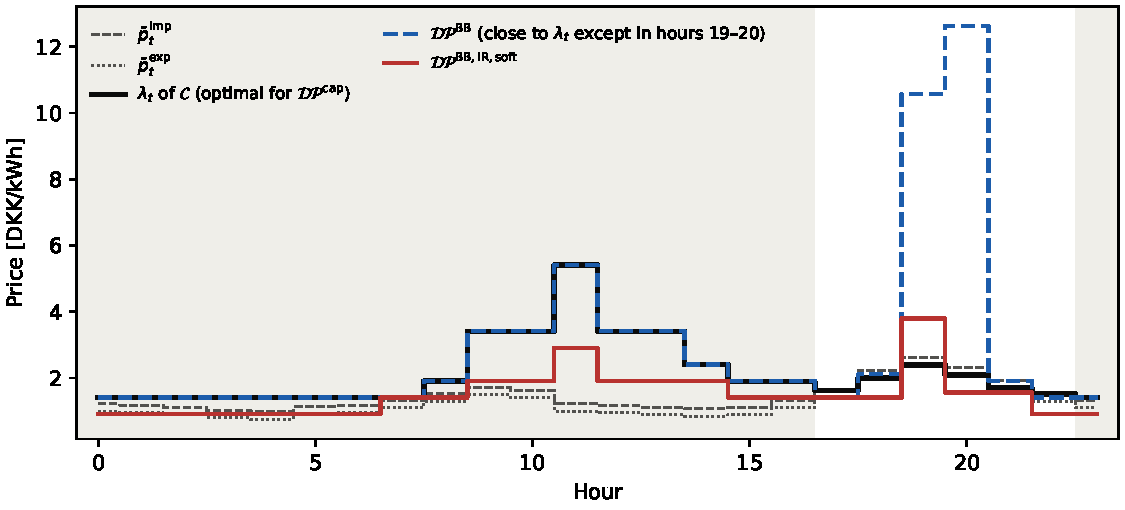
\includegraphics[width=0.85\linewidth]{figures/Q2/q2_prices.pdf}
\caption{Posted prices on the base case (capped hours shaded). Budget balance keeps the prices of $\mathcal{C}$ and returns the rent through two export hours; individual rationality flattens the prices of the capped hours.}
\label{fig:q2_prices}
\end{figure}

\begin{figure}[htbp]
\centering
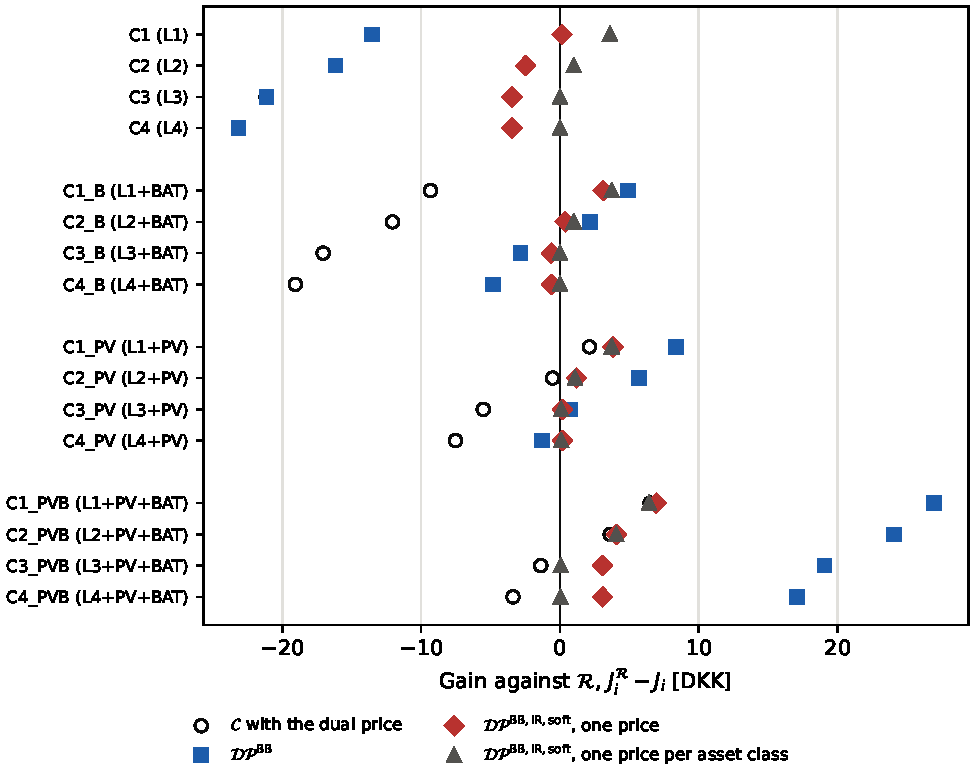
\includegraphics[width=0.72\linewidth]{figures/Q2/q2_members.pdf}
\caption{Gain of every member against $\mathcal{R}$, grouped by assets and ordered by slope. Budget balance alone passes the rent to the PV and battery owners; with one price per asset class nobody is worse off than without a contract.}
\label{fig:q2_members}
\end{figure}

% ---------------------------------------------------------------------------------------------------
\subsection{Indifference}\label{sec:q2_indifference}
% Command: python main.py --q2 indifference
With a linear disutility, a member's best response is a set whenever the price of an hour lies exactly $c^L_i$ away from its internal value $\mu^E_i$.
The optimal prices sit precisely at these points.
In the capped hours, $\lambda_t$ is set by the marginal member.
When a load is marginal, the price equals the night price of 1.41~DKK/kWh plus $2c^L$ of its class (1.91, 2.41, 3.41 and 5.41~DKK/kWh for L1 to L4), because a load only moves a kWh from hour $t$ to hour $s$ if $x_t-x_s>2c^L_i$.
When a battery is marginal, as in hours 15--16, the price is 1.895~DKK/kWh.
At these prices 220 of the 384 member-hours are indifferent, and there are indifferent members in every hour where the cap binds.

The single-level model breaks every one of these ties in the manager's favour, and that is what makes it optimistic.
In practice a member has no reason to choose the schedule the manager has in mind.
If all members broke their ties the other way, hour by hour, the import could exceed the cap in all 18 capped hours, and the manager would pay the penalty $\alpha^{\mathrm{DSO}}$ although every member behaved optimally.
A pessimistic manager would instead price slightly inside each tie, so that every response becomes unique, at a small cost in welfare or budget.
Question~3 returns to this exposure, since with uncertain preferences the members may end up on the wrong side of a tie.

% ---------------------------------------------------------------------------------------------------
\subsection{Sensitivity to the cap}\label{sec:q2_sensitivity}
% Command: python main.py --q2 sensitivity
The base case is a single contract.
Since both requirements are about sharing the congestion rent, the tightness of the cap is the natural dimension to vary (Table~11~c).
We solved the three steps for cap factors $f$ between 1.1 and 4.0, keeping $\beta^{\mathrm{DSO}}=0.75$ and $\alpha^{\mathrm{DSO}}=10$~DKK/kWh fixed (Figure~\ref{fig:q2_sensitivity}).
Before running the study we expected a looser cap to lower the rent, make budget balance cheaper, and turn individual rationality from infeasible into feasible at some threshold.

The results confirm this and place the threshold between $f=1.3$ and $f=1.4$.
From $f=1.4$ on, a single price per hour meets both requirements at no cost in welfare.
The threshold has a clear cause in the merit order of Section~\ref{sec:q2_indifference}.
At $f=1.3$ the cap still forces the stiffest class, L4, to shift 0.4~kWh out of hour 11, which lifts the price of that hour to 5.41~DKK/kWh.
At $f=1.4$ no L4 load needs to move, so the highest price drops to 3.23~DKK/kWh (now set by L3) and the rent halves from 164 to 84~DKK.
The stiff members then pay little enough in the capped hours for one price to leave all of them better off.
Put simply, a uniform price fails as soon as the cap reaches the stiffest members.

Budget balance follows a related logic.
It stays almost free as long as the rent can be handed back through the export hours, where nobody reacts to the price, that is, as long as the rent does not exceed $\sum_t(\overline{x}_t-\lambda_t)P^{\mathrm{exp}}_t$.
In the base case the rent is 164~DKK against a margin of 228~DKK.
At $f=1.2$ the rent of 233~DKK exceeds the margin of 205~DKK, and returning it costs 6.9~DKK of welfare.
This threshold depends on the price bound $\overline{x}_t$, which is therefore a modelling choice with visible consequences.

At the tight end, individual rationality becomes impossible altogether.
Summing~\eqref{eq:DP_IR} over all members under budget balance gives $\sum_is_i\geq J^{\mathcal{DP}}-J^{\mathcal{R}}\geq-V^{\mathcal{C}}$.
At $f=1.1$ the community loses 7.9~DKK even under central dispatch, so no prices, not even one per member, can leave every member better off.
The best uniform price we found there leaves 87~DKK of violation, and every member without PV is blocking.
Prices per asset class reduce the violation considerably, to 23~DKK at $f=1.1$ and 8~DKK at $f=1.2$, and to zero in the base case.
Where the gap is still open, these soft results are the best points found, so they are upper bounds on the smallest possible violation.

\begin{figure}[htbp]
\centering
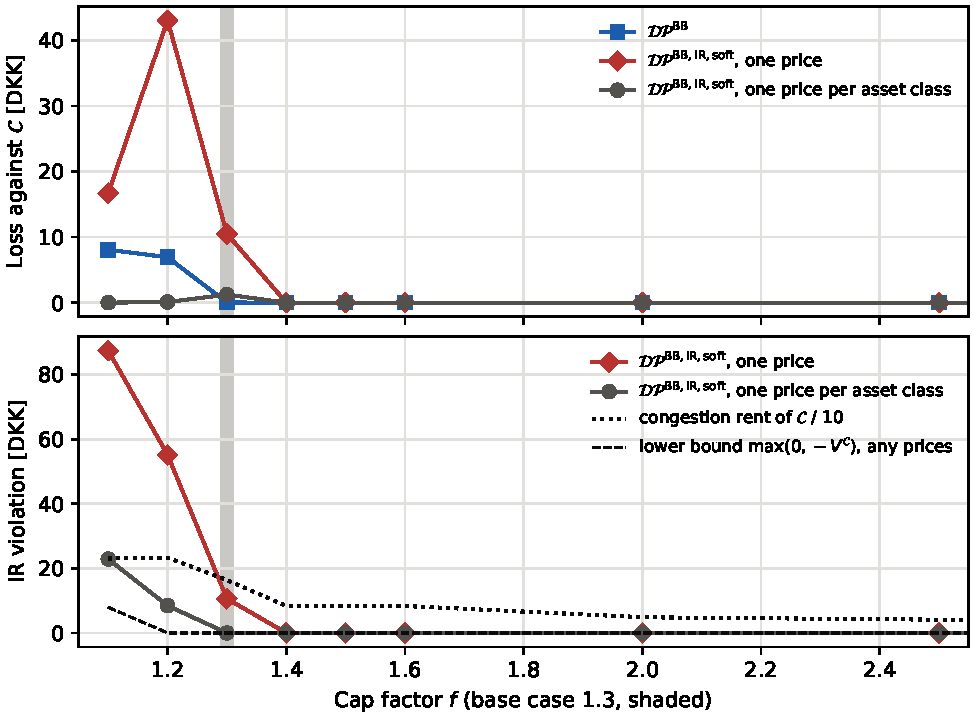
\includegraphics[width=0.75\linewidth]{figures/Q2/q2_sensitivity.pdf}
\caption{Efficiency loss (top) and IR violation (bottom) along the cap factor. One price per hour meets both requirements from $f=1.4$, once the cap no longer forces the stiffest members to move; below $f\approx1.15$ no prices can. Points with $f\leq1.3$ are the best solutions found within 120--240~s; for $f>2.5$ all curves stay at zero.}
\label{fig:q2_sensitivity}
\end{figure}

\subsection{Conclusions and recommendation}
Prices alone can reproduce the central dispatch.
Because the members are price-takers with linear problems, one price per hour recovers the whole value and flexibility of $\mathcal{C}$.
This holds only in the optimistic sense, however: the optimal prices sit on the members' ties, and a manager who cannot count on every tie being broken its way should price slightly inside them.

Of the two requirements, budget balance is almost free in the base case, whereas individual rationality is the one a uniform price struggles with.
The stiff members without PV need low prices in exactly the hours where the flexible members need high ones, and a single price cannot serve both.
In the base case we found no uniform price that leaves every member better off than without a contract.
One price per asset class achieves it for 1.2~DKK of welfare, and one price per member at no cost at all.
Whether a uniform price is enough depends on the contract.
With a loose cap it is, and with a cap so tight that the community as a whole loses, no prices can make every member better off.

We therefore recommend that the manager impose both requirements.
Without them, the price either over-collects, as in Question~1, or hands the rent back to the members who happen to sell in a few export hours.
When the cap is tight, the manager should differentiate the price by asset class, which needs only four price signals and costs little welfare.
For the DSO this is part of the trade-off identified in Question~1: a looser cap makes a simple uniform tariff possible, but removes less congestion.


\newpage
\section{Question 3}
\input{sources/3_}

\newpage
\section{Appendix A} \label{ch6}

All input data of the base cases are those of the repository. The table below lists the values
that were chosen by the group. They are also set in the source code
(\texttt{main.py} and \texttt{src/}), so every result can be reproduced with the commands given in
each section.

\begin{table}[H]
\centering
\small
\begin{tabularx}{\textwidth}{llX}
\toprule
\textbf{Question} & \textbf{Parameter} & \textbf{Chosen values} \\
\midrule
2.(b).iv & Sweep of $c^{L}$ & 0.005 to 3.195~DKK/kWh in steps of 0.01 (offset by 0.005 so that no run lies on a price threshold) \\
2.(c).iv & Sweep of $c^{Q}$ & 0.01 to 3.20~DKK/kWh$^2$ in steps of 0.01 \\
2.(d) & Scenarios & Base: $c^{L} = 1.43$~DKK/kWh, $c^{Q} = 1.00$~DKK/kWh$^2$; low: $c^{L} = c^{Q} = 0.50$; high: $c^{L} = c^{Q} = 3.20$; Question~1 model with $\uL = c^{L}$ \\
2.(e) & Disutility parameters & $\rho = 0.8$, $c^{Q} = 0.05$~DKK/kWh$^2$, $c^{S} = 0.06$~DKK/kWh$^2$ \\
2.(e).iv & Price profiles & Mean of the base prices (1.32~DKK/kWh); flat; alternating $\pm 0.8$~DKK/kWh every hour; blocks of 4~h at $\pm 0.8$~DKK/kWh \\
\midrule
3.(f) & $\Emin$ & 0 to 140~kWh in steps of 5 \\
3.(f) & $c^{Q}$ & 0.1 to 5~DKK/kWh$^2$ in steps of 0.1 (with $\Emin = 40$~kWh) \\
3.(f) & $\Lmax$ & 1.7 to 8~kWh/h in steps of 0.1 (with $\Emin = 40$~kWh) \\
\midrule
3.(g).i & Morning peak of $D+1$ & Searched in hours 0--11 of the following day, \eqref{eq:g_piend} \\
3.(g).v & Price spread & 0, 0.5, 1, 1.5, 2 times the base spread, same mean, on both days \\
3.(g).v & Price level & $-0.5$, 0, 0.5, 1.0~DKK/kWh added to all prices, on both days \\
3.(g).v & $c^{Q}$ & 0.02, 0.1, 0.3, 1, 3, 10~DKK/kWh$^2$ \\
3.(g).v & Capacity $\Ebat$ & 1, 2, 4, 8, 16~kWh, with $\einit$ at 50\,\% of it \\
3.(g).v & Power $\Pch = \Pdis$ & 0.5, 1, 1.5, 3, 6~kW \\
3.(g).v & Efficiency $\etach = \etadis$ & 0.80, 0.85, 0.90, 0.95, 1.00 \\
3.(g).v & End of the day & Trend $\pimp[23] + (\pimp[23] - \pimp[22])$; last price $\pimp[23]$; $\pimp[23]/\etach$; free end; cyclic; $\piend$ from 1.40 to 2.00~DKK/kWh in steps of 0.01 \\
3.(g).v & Benchmark & Day $D$ and hours 0--10 of $D+1$; $\Emin$ on day $D$ only; no value for the energy left at the end \\
\bottomrule
\end{tabularx}
\caption{Values chosen by the group.}
\label{tab:appendix}
\end{table}

% Appendix: KKT conditions and dual objective of the member's problem (Question 2), as implemented in
% src/pricing.py (add_member_kkt). Member index i dropped; t in T; e_{-1} = e^init.
\subsection*{KKT conditions of the member's problem (Question 2)}\label{app:kkt_member}
The duals of~\eqref{eq:DP_member} are $\nu_t$ (free) for~\eqref{eq:dev}, $\mu^E\geq0$ for~\eqref{eq:emin}, $\underline{\mu}^L_t,\overline{\mu}^L_t\geq0$ for the bounds~\eqref{eq:lbounds}, $\underline{\mu}^{\mathrm{PV}}_t,\overline{\mu}^{\mathrm{PV}}_t\geq0$ for~\eqref{eq:pv}, $\psi_t$ (free) for~\eqref{eq:soc}, $\underline{\mu}^{\mathrm{ch}}_t,\overline{\mu}^{\mathrm{ch}}_t,\underline{\mu}^{\mathrm{dis}}_t,\overline{\mu}^{\mathrm{dis}}_t,\underline{\mu}^{e}_t,\overline{\mu}^{e}_t\geq0$ for~\eqref{eq:batbounds} and $\mu^{\mathrm{end}}\geq0$ for~\eqref{eq:eod}.
With $q_t$ substituted by~\eqref{eq:net}, stationarity reads
\begin{align*}
&\ell_t: && x_t-\nu_t-\mu^E-\underline{\mu}^L_t+\overline{\mu}^L_t=0, \qquad
d^{+}_t,\ d^{-}_t:\ \ 0\leq d^{\pm}_t\perp c^L\pm\nu_t\geq0,\\
&q^{\mathrm{PV}}_t: && -x_t+c^{\mathrm{PV}}-\underline{\mu}^{\mathrm{PV}}_t+\overline{\mu}^{\mathrm{PV}}_t=0,\\
&p^{\mathrm{ch}}_t,\ p^{\mathrm{dis}}_t: && x_t+\eta^{\mathrm{ch}}\psi_t-\underline{\mu}^{\mathrm{ch}}_t+\overline{\mu}^{\mathrm{ch}}_t=0, \qquad
-x_t-\psi_t/\eta^{\mathrm{dis}}-\underline{\mu}^{\mathrm{dis}}_t+\overline{\mu}^{\mathrm{dis}}_t=0,\\
&e_t: && -\psi_t+\psi_{t+1}-\underline{\mu}^{e}_t+\overline{\mu}^{e}_t=0\ \ (t<23), \qquad -\psi_{23}-\mu^{\mathrm{end}}-\underline{\mu}^{e}_{23}+\overline{\mu}^{e}_{23}=0,
\end{align*}
together with primal feasibility and the complementarity of every inequality with its dual, e.g.\ $0\leq\ell_t-\ell^{\mathrm{lo}}_t\perp\underline{\mu}^L_t\geq0$ and $0\leq\sum_t\ell_t-E^{\min}\perp\mu^E\geq0$, where $\ell^{\mathrm{lo}}_t$ and $\ell^{\mathrm{up}}_t$ are the two sides of~\eqref{eq:lbounds}.
The dual objective, equal to the member's optimal cost $J^{\mathcal{DP}}_i=\Pi_i+K_i$ by strong duality, is
\begin{multline*}
\Phi=\sum_t\Big(\nu_t\hat{\ell}_t+\underline{\mu}^L_t\ell^{\mathrm{lo}}_t-\overline{\mu}^L_t\ell^{\mathrm{up}}_t-\overline{\mu}^{\mathrm{PV}}_tPV^{\max}_t\Big)\\
-\sum_t\Big(\overline{\mu}^{\mathrm{ch}}_tP^{\mathrm{ch}}+\overline{\mu}^{\mathrm{dis}}_tP^{\mathrm{dis}}+\overline{\mu}^{e}_tE^{\mathrm{bat}}\Big)+\mu^EE^{\min}+(\psi_0+\mu^{\mathrm{end}})\,e^{\mathrm{init}} .
\end{multline*}
It contains no price, which is why it linearizes the payments in~\eqref{eq:DP_BB} and~\eqref{eq:DP_IR}.

\paragraph{Big-M constants.}
Each complementarity pair $0\leq a\perp b\geq0$ becomes $a\leq M^{\mathrm{P}}u$, $b\leq M^{\mathrm{D}}(1-u)$ with $u$ binary.
The primal constants follow from $\mathcal{X}_i$ (e.g.\ $M^{\mathrm{P}}=\ell^{\mathrm{up}}_t-\ell^{\mathrm{lo}}_t$ for the load bounds).
For the load and the PV, the dual constants are not guessed but derived from the conditions above, given $0\leq x_t\leq\overline{x}$.
Dual feasibility of $d^{\pm}_t$ gives $|\nu_t|\leq c^L$, so both reduced costs lie in $[0,2c^L]$.
If $\mu^E$ exceeded $\overline{x}+c^L$, stationarity would force $\overline{\mu}^L_t>0$, hence $\ell_t=\ell^{\mathrm{up}}_t$, in every hour, and the daily minimum would be slack, contradicting $\mu^E>0$; therefore $\mu^E\leq\overline{x}+c^L$.
Since the two bounds of $\ell_t$ never coincide, at most one of their duals is positive, which gives $\underline{\mu}^L_t\leq\overline{x}+c^L$ and $\overline{\mu}^L_t\leq\overline{x}+2c^L$.
In the same way $\underline{\mu}^{\mathrm{PV}}_t\leq c^{\mathrm{PV}}$ and $\overline{\mu}^{\mathrm{PV}}_t\leq\overline{x}-c^{\mathrm{PV}}$.
These bounds hold at every KKT point, so they cut off no response.
The battery duals use the generic constant $M^{\mathrm{D}}=50$~DKK/kWh, and after each solve we check that none of them reaches it.



\label{endOfDoc}
\label{EndOfText}
\end{document}
